%\lipsum[4-4]

In this chapter, the system specification is defined, starting with the overview of the existing communication systems and defining the SRS. After that is made a market survey on the existing technologies and raised the protocols, standards and communication KPI's.



\section{Overview of the existing wireless communication system}
%\lipsum[4]
In the attachment 1 is presented a work that highlights the communication systems for energy metering systems used in smart meters. On the field of the wireless technologies we can list the following technologies to be applied in this work:

\begin{itemize}
	\setlength\itemsep{-0.5em}
	\item IEEE 802.15.4 (ZigBee);
	\item DASH7;
	\item IEEE 802.11 (Wireless LAN (WLAN) or Wi-Fi);
	\item IEEE 802.16 (WIMAX);
	\item GSM or GPRS;
	\item LTE/LTE-Advanced.	
\end{itemize}

For the purpose of this work, the usage of medium distances is advantageous (on distances of hundreds of meters). Complementary, solutions that depends on a service provided by a communication enterprise is not interesting. 


The research areas of interest on the WSNs in the last decade are the following:

\begin{itemize}
	\setlength\itemsep{-0.5em}
	\item Propagation characteristics \& channel modeling
	\item Protocols design (routing, MAC)
	\item Energy conservation
	\item Security
	\item Topology Control

\end{itemize}

\section{System Requirement Specification}
%\lipsum[1-4]
In the attachment 2 is present the SRS document. This document uses the following structure (based on a template from Generic Ethernet Gateway (GWAY) developed by Chrysler Group LLC):
\begin{description}
	\item[Introduction] This part describes the purpose of the document, the scope and the context of the system/project where is implemented;
	
	\item[Overall Description] In this part is described the system, it's objectives and features as well as some design and implementation constraints;
	
	\item[Specific requirements] This part defines the specification of the requirements that the system must comply with;
	
	\item[Data Model and Description] This part covers the definition of the system in UML diagrams and descriptions.
			
\end{description}

The definition of the system with this document allows the system specification according to the main goal of this activity: the development of a Wireless network to monitor existent PV power converters.

\section{Market	survey on wireless technologies}
The market survey was conducted to cover recent technologies among manufacturers with enhanced market share.

\subsection{Atmel -- SAM R21 Xplained Pro Evaluation Kit}



\begin{framed}

	http://www.atmel.com/tools/atsamr21-xpro.aspx
\vspace{1em}
%	\hline
\vspace{1em}
\small
\textit{The Atmel® SAM R21 Xplained Pro evaluation kit is a hardware platform to evaluate the ATSAMR21G18A microcontroller. Supported by the Atmel Studio integrated development platform, the kit provides easy access to the features of the Atmel ATSAMR21G18A and explains how to integrate the device in a custom design. The Xplained Pro MCU series evaluation kits include an on-board Embedded Debugger, and no external tools are necessary to program or debug the ATSAMR21G18A. The Xplained Pro extension kits offers additional peripherals to extend the features of the board and ease the development of custom designs.}
\end{framed}

In synthesis, this platform is based on a single chip solution that integrates in the same integrated circuit an ARM® Cortex®-M0+ processor and an integrated ultra-low-power 2.4GHz ISM
band transceiver. It's relevance is on the ultra-low-power consumption (less that 70$\mu$A in active mode and less than 3.5$\mu$A in sleep mode).

\begin{figure}[h!]
	\centering
	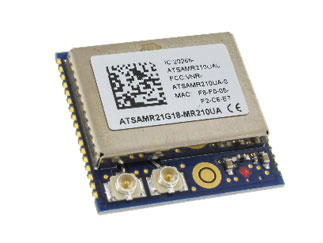
\includegraphics[width=0.35\textwidth,keepaspectratio]{figures/samr21}
	\caption{SAM R21 Xplained Pro module.}

\end{figure}

%%%%%%%%%%%%%%%%%%%%%%%%%%%%%%%

\subsection{CC1310 SimpleLink™ Sub-1 GHz Ultra-Low Power Wireless Microcontroller}

\begin{framed}
	
	http://www.ti.com/product/CC1310
	
	\vspace{1em}
%	\hline
	\vspace{1em}
\small	
	\textit{The CC1310 is a member of the CC26xx and CC13xx family of cost-effective, ultra-low-power, 2.4-GHz and Sub-1 GHz RF devices. Very low active RF and microcontroller (MCU) current consumption, in addition to flexible low-power modes, provide excellent battery lifetime and allow long-range operation on small coin-cell batteries and in energy-harvesting applications.}
		
	\textit{The CC1310 device is the first device in a Sub-1 GHz family of cost-effective, ultra-low-power wireless MCUs. The CC1310 device combines a flexible, very low power RF transceiver with a powerful 48-MHz Cortex®-M3 microcontroller in a platform supporting multiple physical layers and RF standards. A dedicated Radio Controller (Cortex®-M0) handles low-level RF protocol commands that are stored in ROM or RAM, thus ensuring ultra-low power and flexibility. The low-power consumption of the CC1310 device does not come at the expense of RF performance; the CC1310 device has excellent sensitivity and robustness (selectivity and blocking) performance.}
		
\end{framed}




\vspace{-1.5em}
\begin{figure}[h!]
	\centering
	\begin{minipage}{.5\textwidth}
		\centering
		\vspace{2.5em}
		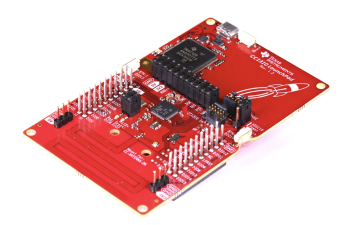
\includegraphics[width=1\textwidth,keepaspectratio]{figures/cc1310_board}
		\vspace{2em}
		\captionof{figure}{CC1310 evaluation board.}
		\label{fig:test1}
	\end{minipage}%
	\begin{minipage}{.5\textwidth}
		\centering
		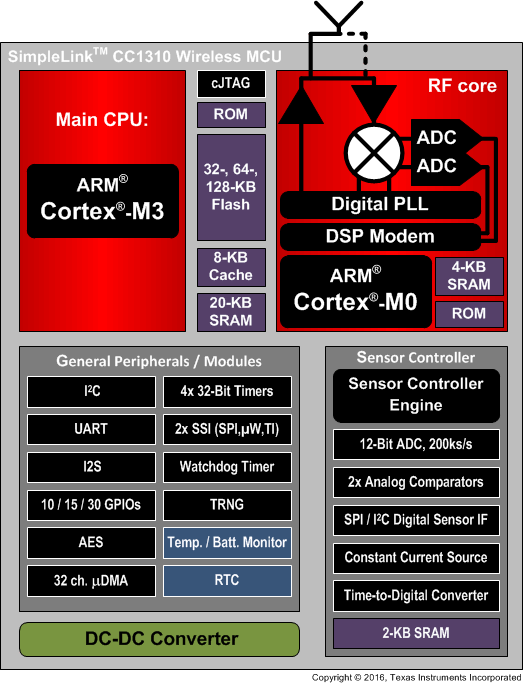
\includegraphics[width=0.70\textwidth,keepaspectratio]{figures/cc1310}
		\captionof{figure}{CC1310 chip architecture.}
		\label{fig:test2}
	\end{minipage}
\end{figure}
The CC1310 is a Texas Instruments platform launched to operate the sub-GHz frequency band. It depends on a ARM® Cortex®-M3 processor and an integrated ultra-low-power RF Core. It is integrated in the category of "Wireless MCU's" due to it's integration of CPU and RF core, similarly to the Atmel SAM-R21 previoulsy presented platform.


%%%%%%%%%%%%%%%%%%%%%%%%%%%

\subsection{Adafruit Feather 32u4 Radio (RFM69HCW)}

\begin{framed}
	
	https://learn.adafruit.com/adafruit-feather-32u4-radio-with-rfm69hcw-module/overview
	
	\vspace{1em}
%	\hline
	\vspace{1em}
\small	
	\textit{This Adafruit Feather 32u4 Radio (RFM69HCW) 900MHz microcontroller packet radio transceiver with built in USB and battery charging. 32u4 with a 900MHz radio module cooked in an Adafruit Feather. Great for making wireless networks that can go further than 2.4GHz 802.15.4 and similar, are more flexible than Bluetooth LE and without the high power requirements of WiFi. The 900MHz radio version can be used for either 868MHz or 915MHz transmission/reception. At the Feather, 32u4's heart is at ATmega32u4 clocked at 8MHz and at 3.3V logic. This chip has 32K of flash and 2K of RAM, with built in USB so not only does it have a USB-to-Serial program and debug capability built in with no need for an FTDI-like chip, it can also act like a mouse, keyboard, USB MIDI device, etc.}
\end{framed}

%%%%%%%%%%%%%%%%%%%%%%%%%%%

\subsection{Adafruit Feather HUZZAH ESP8266}

\begin{framed}
	
	https://learn.adafruit.com/adafruit-feather-huzzah-esp8266/overview
	
	\vspace{1em}
%	\hline
	\vspace{1em}
\small	
	\textit{This is the Adafruit Feather HUZZAH ESP8266 - our take on an 'all-in-one' ESP8266 WiFi development board with built in USB and battery charging. At the Feather HUZZAH's heart is an ESP8266 WiFi microcontroller clocked at 80 MHz and at 3.3V logic. This microcontroller contains a Tensilica chip core as well as a full WiFi stack. You can program the microcontroller using the Arduino IDE for an easy-to-run Internet of Things core. We wired up a high-quality SiLabs CP2104 USB-Serial chip that can upload code at a blistering 921600 baud for fast development time. It also has auto-reset so no noodling with pins and reset button pressings. The CP2104 has better driver support than the CH340 and can do very high speeds without stability issues.}
\end{framed}

%%%%%%%%%%%%%%%%%%%%%%%%%%%

\vspace{-1em}
\begin{figure}[h!]
	\centering
	\begin{minipage}{.47\textwidth}
		\centering

		\includegraphics[width=0.90\textwidth,keepaspectratio]{figures/feather_3077}

		\captionof{figure}{Adafruit Feather 32u4 Radio (RFM69HCW).}
		\label{fig:test3}
	\end{minipage}%
	\begin{minipage}{.05\textwidth}
		\centering
		~
	\end{minipage}%	
	\begin{minipage}{.47\textwidth}
		\centering
		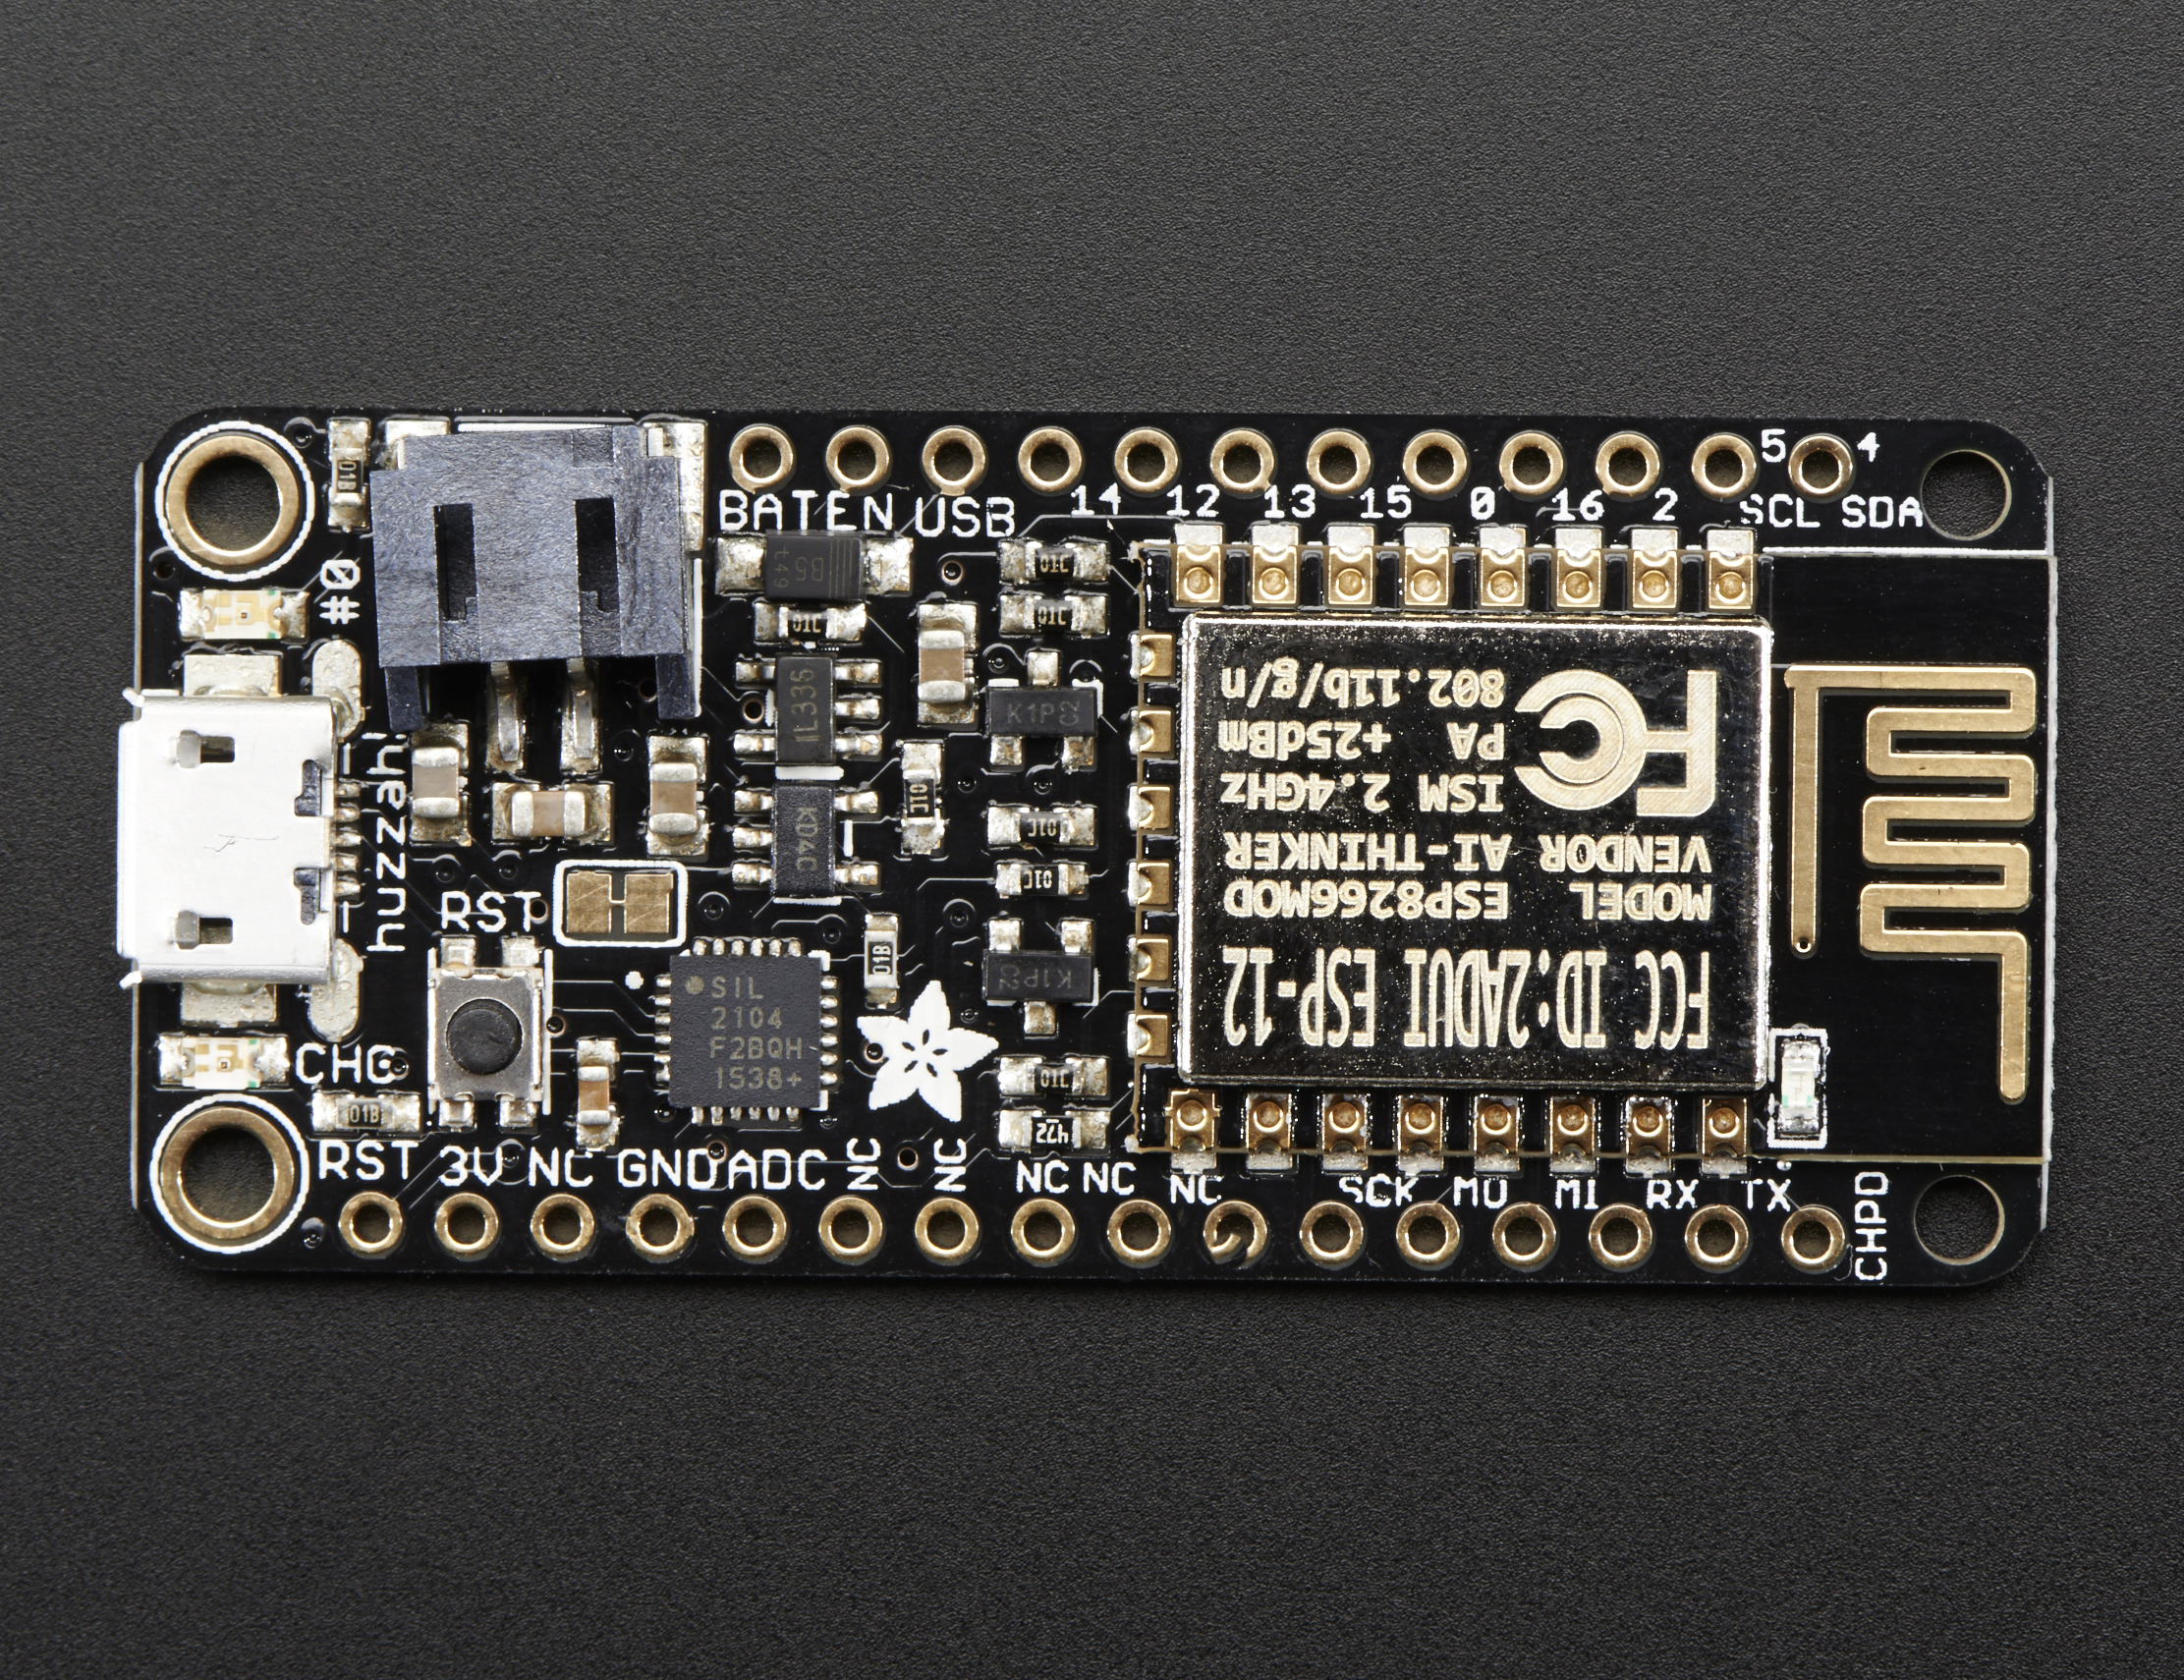
\includegraphics[width=0.90\textwidth,keepaspectratio]{figures/feather_wifi}
		\captionof{figure}{Adafruit Feather HUZZAH ESP8266.}
		\label{fig:test4}
	\end{minipage}
\end{figure}

Both Adafruit Feather modules (for sub-GHz and for WiFi) are designed for cheap and modular solutions.

\subsection{ATxmega256A3U AT86RF233 ZigBit Module}

\begin{framed}
	
	http://www.atmel.com/pt/br/devices/ATxmega256A3U-and-AT86RF233-ZigBit-Wireless-Module.aspx
	
	\vspace{1em}
%	\hline
	\vspace{1em}
\small	
	\textit{The Atmel ZigBit 2.4GHz ATZB-X0-256-3-0-C wireless system-on-module is designed to work with IEEE 802.15.4 and ZigBee WPAN communication protocols. The ZigBit module is compatible with a ZigBee stack that supports a self-healing, self-organizing mesh network, while optimizing network traffic and minimizing power consumption.}
\end{framed}

\begin{figure}[h!]
	\centering
	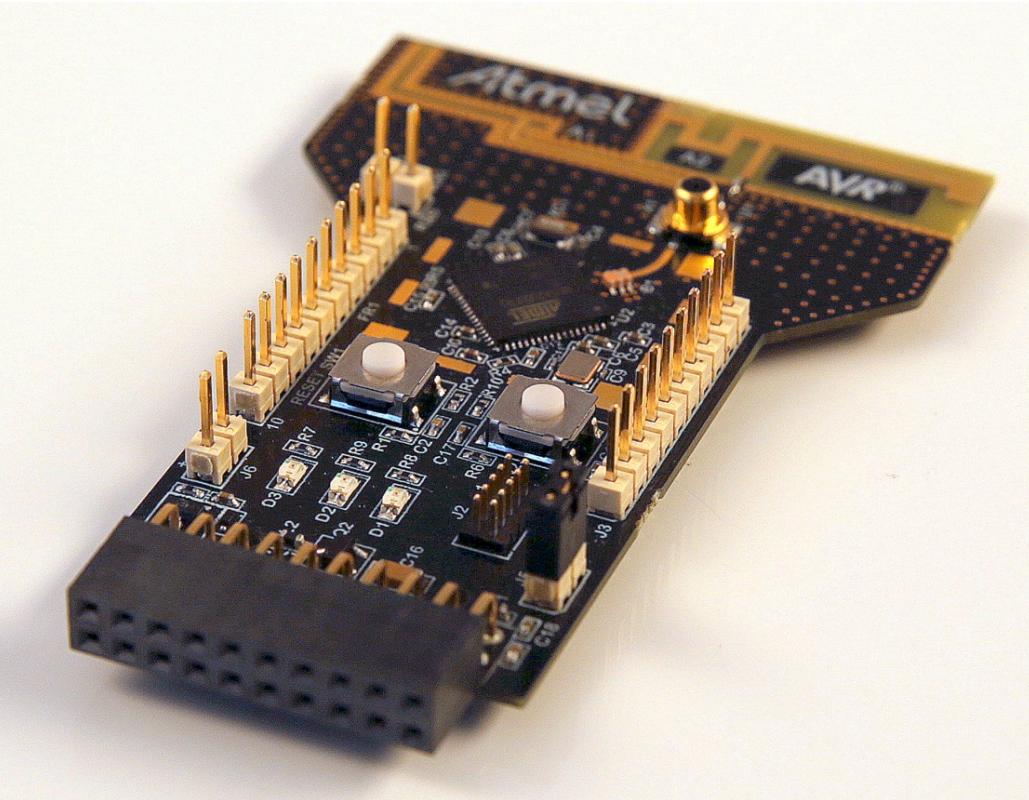
\includegraphics[width=0.35\textwidth,keepaspectratio]{figures/atxmega}
	\caption{ATxmega256A3U AT86RF233 ZigBit Module.}
	
\end{figure}

%%%%%%%%%%%%%%%%%%%%%%%%%%

\subsection{CC1350 SimpleLink™ Ultra-Low Power Dual Band Wireless Microcontroller}

\begin{framed}
	
	http://www.atmel.com/pt/br/devices/ATxmega256A3U-and-AT86RF233-ZigBit-Wireless-Module.aspx
	
	\vspace{1em}
%	\hline
	\vspace{1em}
\small	
	\textit{The CC1350 is a member of the CC26xx and CC13xx family of cost-effective, ultra-low-power, 2.4-GHz and Sub-1 GHz RF devices from Texas Instruments™. Very low active RF and microcontroller (MCU) current consumption, in addition to flexible low-power modes, provide excellent battery lifetime and allow long-range operation on small coin-cell batteries and in energy-harvesting applications.}
		
		\textit{The CC1350 is the first device in the CC13xx and CC26xx family of cost-effective, ultra-low-power wireless MCUs capable of handling both Sub-1 GHz and 2.4-GHz RF frequencies. The CC1350 device combines a flexible, very low-power RF transceiver with a powerful 48-MHz ARM® Cortex®-M3 microcontroller in a platform supporting multiple physical layers and RF standards. A dedicated Radio Controller (Cortex®-M0) handles low-level RF protocol commands that are stored in ROM or RAM, thus ensuring ultra-low power and flexibility to handle both Sub-1 GHz protocols and 2.4 GHz protocols (for example Bluetooth® low energy). This enables the combination of a Sub-1 GHz communication solution that offers the best possible RF range together with a Bluetooth low energy smartphone connection that enables great user experience through a phone application. The Sub-1 GHz only device in this family is the CC1310.}
\end{framed}

This CC1350 adds the Bluetooth® low energy functionality to the CC1310 module with small increase on the cost of the solution. 

\section{Protocols and standards}
%\lipsum[4]

In computer networks, a protocol is a set of rules that ensure a communication of specific set of information between two machines. A standard is a document that specifies several aspects of something that has the overwhelming agreement and support of a entity (the standards making body). In the networking area, several protocols are supported by standards. In this section is presented some of the protocols that ensure a coherent communication among the sensor networks.

\subsection{IEEE 802.15}

The standard family defines the topologies and network roles. In particular, it defines the physical (frequency and channels, spectrum handling, modulation and bit rate) and MAC (packet formats, operational modes, timing aspects, topologies) layers of the OSI model (\cite{Hackmann2006}).


\begin{figure}[h!]
	\centering
	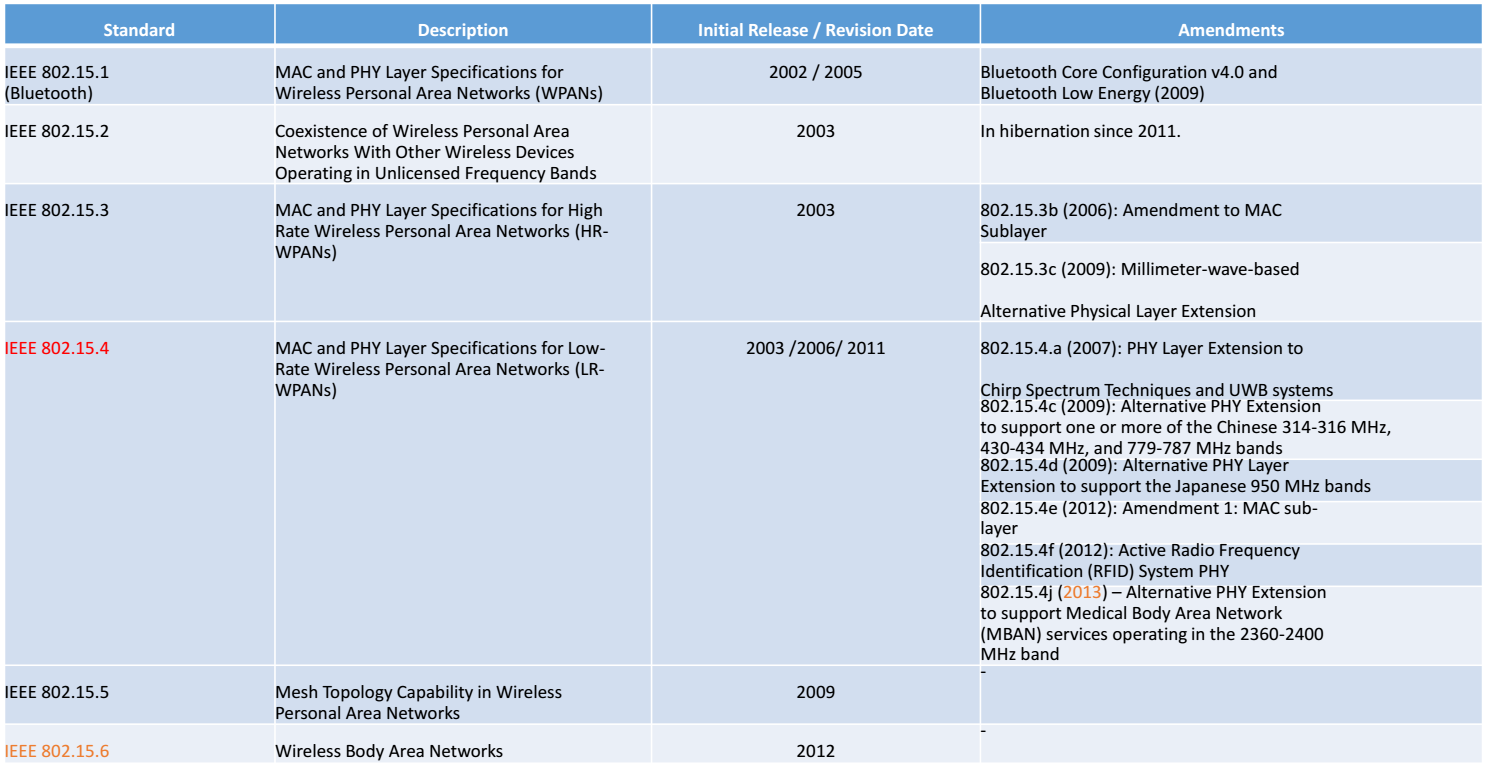
\includegraphics[width=1.1\textwidth,keepaspectratio]{figures/nancy2014}
	\caption{Members of the 802.15 family. Adapted from \cite{nancy2014} lecture presentation slides.}
	\label{fig:nancy2014}
\end{figure}

Based on figure \ref{fig:nancy2014}, the 802.15.4 is the standard that defines the PHY and MAC layers for low rate wireless personal area networks. It supports \textbf{full-function devices} (device capable of being the network coordinator or simple node and can have implemented complex network functionalities) and \textbf{reduced-function device} (limited devices with low-bandwidth limitations and limited or no-network intelligence). The possible network topologies are the following:

\begin{description}
	\item[Star ---] Each device in the network communicates with the full-function device network coordinator;
	
	\item[Peer-to-peer ---] All devices communicate with each others (if they are in the communication range). Sufficiently flexible to implement more complex topologies such as multi-hoping, cluster trees and mesh topologies;
	
	\item[Multi-hopping ---] This is a technique that allows the usage of two or more wireless nodes to convey data from a source to a destination;
	
	\item[Cluster trees] Topology to reduce the routing complexity where each node knows its parent node and all it's child nodes. It has always only one single path between two nodes.
	
	\item[Wireless mesh] This technique allows data to be propagated along a path by hopping from node to node until it reaches its destination.
		
\end{description}

\subsection{802.15.4-based wireless standards}

\cite{Radmand2010} presents a comparison of wireless sensor standards for industrial applications. In figure \ref{fig:randmand2010} is present the overall schema of the wireless standards.


\begin{figure}[h!]
	\centering
	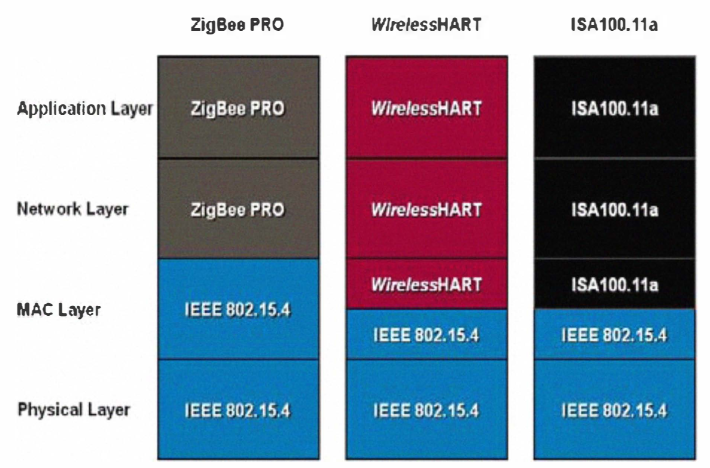
\includegraphics[width=0.6\textwidth,keepaspectratio]{figures/radmand2010}
	\caption{Overall schema of wireless standards. Adapted from \cite{Radmand2010}.}
	\label{fig:radmand2010}
\end{figure}


\section{Communication KPI’s}
%\lipsum[4]

According to \cite{Radmand2010}, it is identified the following "Industrial Requirements" for the WSN's:

\begin{description}
	\item[Reliability ---] Reliability is a measurement of the transmission accuracy, in percentage, that evaluates the amount of data that reach it's destination. This measurement uses the properties of data communication, acknowledge-based usually.
	
	\item[Latency ---] Latency is the measurement of the time delay and is defined as the time that a data packet takes to be transmited from the source to the destination. The latency is directly related to the link quality and a high latency link is result of a link with high signal-to-noise ratio. 
	
	\item[Sensor Data Update Rates ---] This KPI is not directly related with the communication link. However the update rate of the sensor data affects the power consumption due to the increase of the processing effort. In a SYNC-based update rate, this KPI is related to the frequency of the SYNC event.
	
	\item[Wireless Transmission Range ---] This KPI is the the maximum distance that a communication link supports the data transfer with a given reliability and in specific conditions (indoor/outdoor; line-of-sight or LOS).
	
	\item[Power consumption ---] The power consumption is a measurement of the combination of the computational effort of the nodes and the transmission effort. It is directly related with the update rate as well as with the link quality and, if it exists, the routing activity in each node.

\end{description}







